\subsection{\texorpdfstring{\(\tau\)-扩张的逆像}{\textbackslash tau-扩张的逆像}}

设 G 与 \(G'\) 是群。设 F 是一个交换群，并设 \(\tau: G \to \text{Aut}(F)\) 与 \(u: G' \to G\) 是群同态。考虑群同态 \(\tau' = \tau \circ u: G' \to \text{Aut}(F)\)，并用 \(\Gamma'\) 表示纤维积 \(\Gamma \times_{G} G'\)（关于 \(\pi\) 与 u 的）（I, §4, No.~8, 第 46 页）。它是 \(\Gamma \times G'\) 的由偶 \((\gamma, g')\) 组成的子群，这些偶满足 \(\pi(\gamma) = u(g')\)。设 \(\iota': F \to \Gamma'\) 是由 \(\iota'(\alpha) = (\iota(\alpha), e)\)（对 \(\alpha \in F\)）给出的群同态，并用 \(\pi': \Gamma' \to G'\) 表示第二个投影。则态射 \(\iota'\) 是单射的，态射 \(\pi'\) 由于 \(\pi\) 是满射的而也是满射的，且 \(\iota'\) 的像与 \(\pi'\) 的核重合。此外，对每个 \(\alpha \in F\) 与 \(\gamma' = (\gamma, g) \in \Gamma'\)，我们有关系

\[
\gamma^ {\prime} \iota^ {\prime} (\alpha) \gamma^ {- 1} = (\gamma , g) (\iota (\alpha), e) (\gamma , g) ^ {- 1} = (\iota (\tau (\pi (\gamma)). \alpha), e) = \iota^ {\prime} (\tau^ {\prime} (\pi^ {\prime} (\gamma^ {\prime})). \alpha)
\]

于是，\((\Gamma', \iota', \pi')\) 是一个 \(\tau'\)-扩张（\(G'\) 被 F 的）；我们称它为 E 被 u 的逆像，并记作 \(u^{*}(\mathcal{E})\)。第一个投影是一个群同态 \(\varphi : \Gamma' \to \Gamma\)，我们称之为典范的。

命题 1. —— 下面的图交换：

\[
\begin{array}{c} \mathrm{F} \xrightarrow {\iota^ {\prime}} \Gamma^ {\prime} \xrightarrow {\pi^ {\prime}} \mathrm{G} ^ {\prime} \\ \Big \| \qquad \qquad \qquad \Big \downarrow \varphi \qquad \qquad \Big \downarrow u \\ \mathrm{F} \xrightarrow {\iota} \Gamma \xrightarrow {\pi} \mathrm{G}. \end{array}\tag{2}
\]

此外，若 \(\mathcal{E}_1' = (\Gamma_1', \iota_1', \pi_1')\) 是一个 \(\tau'\)-扩张，且 \(\varphi_1: \Gamma_1' \to \Gamma\) 是一个使得图

\[
\begin{array}{c} \mathrm{F} \xrightarrow {\iota_ {1} ^ {\prime}} \Gamma_ {1} ^ {\prime} \xrightarrow {\pi_ {1} ^ {\prime}} \mathrm{G} ^ {\prime} \\ \Big \| \qquad \qquad \qquad \Big \downarrow \varphi_ {1} \qquad \qquad \Big \downarrow u \\ \mathrm{F} \xrightarrow {\iota} \Gamma \xrightarrow {\pi} \mathrm{G} \end{array}
\]

交换的群同态，则存在唯一的态射 \(\psi\)（\(\tau'\)-扩张的、从 \(\mathcal{E}_1'\) 到 \(u^*(\mathcal{E})\) 的），使得我们有 \(\varphi_1 = \varphi \circ \psi\)。

第一个图的交换性由 \(\varphi\) 的定义得出。\(\psi\) 的存在性与唯一性由下面的引理 2 得出。

引理 2. —— 设 \(F_{1}^{\prime}\) 是一个交换群，并设 \(w : F_{1}^{\prime} \to F\) 与 \(\tau_{1}: G^{\prime} \to \operatorname{Aut}(F_{1}^{\prime})\) 是群同态，使得

\[
w (\tau_ {1} (g) (f)) = \tau (u (g)) (w (f))
\]

（对每个 \(f \in \mathrm{F}_1'\) 与 \(g \in \mathrm{G}'\)）。设 \(\mathcal{E}_1' = (\Gamma_1', \iota_1', \pi_1')\) 是一个 \(\tau_1\)-扩张（\(\mathrm{G}'\) 被 \(\mathrm{F}_1'\) 的），且 \(\varphi_1: \Gamma_1' \to \Gamma\) 是一个使下图交换的群同态：

\pandocbounded{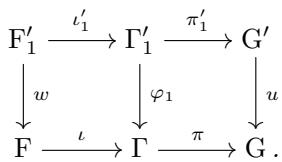
\includegraphics[keepaspectratio]{images/part002_e5b6b945.jpg}}

则存在唯一的群同态 \(\psi : \Gamma_1' \to \Gamma'\)，使得图

\pandocbounded{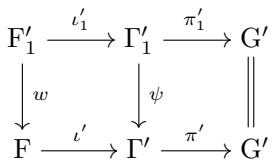
\includegraphics[keepaspectratio]{images/part002_7bcd6e81.jpg}}

交换且 \(\varphi_{1} = \varphi \circ \psi\)。

若群同态 \(\psi : \Gamma_1' \to \Gamma'\) 具有所要的性质，则它满足关系

\[
\psi (\gamma) = (\varphi \circ \psi (\gamma), \pi^ {\prime} \circ \psi (\gamma)) = (\varphi_ {1} (\gamma), \pi_ {1} ^ {\prime} (\gamma))
\]

（对每个 \(\gamma \in \Gamma_1'\)）。反之，从 \(\Gamma_1'\) 到 \(\Gamma \times G'\) 的由 \(\gamma \mapsto (\varphi_1(\gamma), \pi_1'(\gamma))\) 定义的群同态取值在纤维积 \(\Gamma \times_G G'\) 中，因为 \(\pi \circ \varphi_1(\gamma) = u \circ \pi_1'(\gamma)\)（对每个 \(\gamma \in \Gamma_1'\)）。

推论 1. —— 设 \(E_{1}\) 与 \(E_{2}\) 是 G 被 F 的 \(\tau\)-扩张，并设 \(\psi\) 是一个 \(\tau\)-扩张的态射（从 \(E_{1}\) 到 \(E_{2}\) 的）。用 \(\varphi_{1}\)（相应地，\(\varphi_{2}\)）表示 \(u^{*}(\mathcal{E}_{1})\)（相应地，\(u^{*}(\mathcal{E}_{2})\)）的典范同态。则存在唯一的 \(\tau'\)-扩张的态射（从 \(u^{*}(\mathcal{E}_{1})\) 到 \(u^{*}(\mathcal{E}_{2})\) 的），记作 \(u^{*}(\psi)\)，使得 \(\varphi_{2} \circ u^{*}(\psi) = \psi \circ \varphi_{1}\)。

只需对 \(\psi \circ \varphi_{1}\) 应用命题 1。

于是 \(\tau^{\prime}\)-扩张 \(u^{*}(\mathcal{E})\) 的类只依赖于 E 的类。我们也用 \(u^{*}:\operatorname{Ex}_{\tau}(\mathrm{G},\mathrm{F})\to\operatorname{Ex}_{\tau^{\prime}}(\mathrm{G}^{\prime},\mathrm{F})\) 表示把一个 \(\tau\)-扩张 E 的类映到 \(\tau^{\prime}\)-扩张 \(u^{*}(\mathcal{E})\) 的类的映射。

推论 2. —— 设 \(u': G'' \to G'\) 是一个群同态，\(\mathcal{E}\) 是 G 被 F 的一个 \(\tau\)-扩张。设 \(\tau'' = \tau' \circ u'\)，并用 \(\varphi\)（相应地，\(\varphi', \varphi''\)）表示与 \(\tau'\)-扩张 \(u^*(\mathcal{E})\)（相应地，\(\tau''\)-扩张 \(u'^*(u^*(\mathcal{E}))\)、\(\tau''\)-扩张 \((u \circ u')^*(\mathcal{E})\)）相伴的典范同态。则存在唯一的态射 \(\psi\)（从 \(\tau''\)-扩张 \(u'^*(u^*(\mathcal{E}))\) 到 \(\tau''\)-扩张 \((u \circ u')^*(\mathcal{E})\) 的），使得 \(\varphi'' \circ \psi = \varphi \circ \varphi'\)。

例. —— 设 H 是 G 的一个子群，\(j : H \to G\) 是典范单射。则对每个 \(\tau\)-扩张 \(\mathcal{E} = (\Gamma, \iota, \pi)\)，\(\tau \circ j\)-扩张 \(j^{*}(\mathcal{E})\) 同构于 \((\bar{\pi}^{1}(H), \iota', \pi')\)，其中 \(\iota' : F \to \bar{\pi}^{1}(H)\)（相应地，\(\pi' : \bar{\pi}^{1}(H) \to H\)）是群同态 \(f \mapsto \iota(f)\)（相应地，\(\gamma \mapsto \pi(\gamma)\)）。更一般地，若群同态 \(u : G' \to G\) 是单射的，则典范同态 \(\varphi\) 是单射的，其像为 \(\bar{\pi}^{1}(u(G'))\)。
% semantic-fragments: legacy-input-seam
\relax{}
